%----------------------------------------------------------------------------------------
% METADATA BLOCK (YAML)  — see inbox/README.md
%----------------------------------------------------------------------------------------
% uid: ""
% school: "lycee"
% level: "3eme"
% section: "Economie et Gestion"
% chapter: "Statistiques"
% title: "Chiffre d'affaires d'une boutique en ligne"
% difficulty: "Facile"
% tags: ["statistiques", "serie-double", "droite-de-mayer", "prevision"]
% provenance: "own"
% batch: "2026-11-19-3eco-statistiques-n5"
%----------------------------------------------------------------------------------------

\newcommand{\R}{\mathbb{R}}
\newcommand{\vect}[1]{\overrightarrow{#1}}

% ---STATEMENT---
Chiffre d'affaires $y$ (en milliers de dinars) d'une boutique en ligne au cours de ses six premiers mois ($x$ est le rang du mois) :
\begin{center}
\begin{tabular}{|l|c|c|c|c|c|c|}\hline
Rang $x_i$ & $1$ & $2$ & $3$ & $4$ & $5$ & $6$ \\\hline
$y_i$ & $7$ & $8$ & $12$ & $16$ & $17$ & $21$ \\\hline
\end{tabular}\end{center}
\begin{enumerate}
  \item Représenter le nuage de points et calculer les coordonnées du point moyen $G$.
  \item Soient $G_1$ le point moyen des trois premiers points et $G_2$ celui des trois derniers. Calculer leurs coordonnées.
  \item Montrer qu'une équation de la droite $(G_1G_2)$ est $y=3x+3$, puis vérifier que $G$ appartient à cette droite.
  \item En utilisant cet ajustement, estimer le chiffre d'affaires du $9^{\text{e}}$ mois.
  \item À partir de quel mois peut-on prévoir un chiffre d'affaires supérieur à $40$ milliers de dinars ?
\end{enumerate}

% ---SOLUTION---
\begin{enumerate}[itemsep=14pt]
  \item
  \begin{center}
% alt: Nuage de six points croissant, points moyens G1(2 ; 9), G2(5 ; 18), G(3,5 ; 13,5) et droite y = 3x + 3.
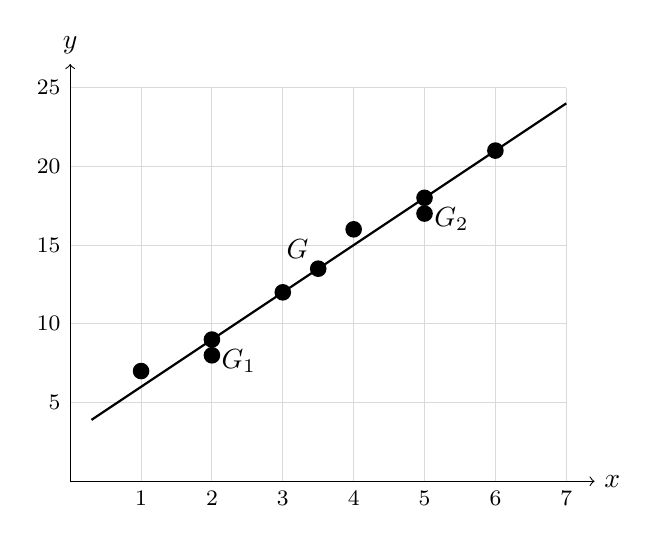
\begin{tikzpicture}[x=0.9cm,y=0.2cm]
    \draw[gray!30] (0,0) grid[xstep=1,ystep=5] (7,25);
    \draw[->] (0,0)--(7.4,0) node[right]{$x$};
    \draw[->] (0,0)--(0,26.5) node[above]{$y$};
    \foreach \x in {1,...,7} \node[below] at (\x,0) {\footnotesize\x};
    \foreach \y in {5,10,...,25} \node[left] at (0,\y) {\footnotesize\y};
    \draw[thick] (0.3,3.9)--(7,24);
    \foreach \x/\y in {1/7,2/8,3/12,4/16,5/17,6/21} \fill (\x,\y) circle (3pt);
    \fill[black] (3.5,13.5) circle (3pt) node[above left]{$G$};
    \fill[black] (2,9) circle (3pt) node[below right]{$G_1$} (5,18) circle (3pt) node[below right]{$G_2$};
  \end{tikzpicture}
  \end{center}
  \[\overline x=\dfrac{1+2+3+4+5+6}{6}=\dfrac{21}{6}=3{,}5\qquad\overline y=\dfrac{7+8+12+16+17+21}{6}=\dfrac{81}{6}=13{,}5\]
  \[G(3{,}5\,;13{,}5)\]

  \item
  \[G_1\left(\dfrac{1+2+3}{3}\,;\dfrac{7+8+12}{3}\right)=(2\,;9)\qquad G_2\left(\dfrac{4+5+6}{3}\,;\dfrac{16+17+21}{3}\right)=(5\,;18)\]

  \item
  \begin{prop}[Droite passant par deux points]
  Le coefficient directeur de $(G_1G_2)$ est \ib{$a=\dfrac{y_{G_2}-y_{G_1}}{x_{G_2}-x_{G_1}}$}, puis on trouve $b$ en écrivant que $G_1$ est sur la droite $y=ax+b$.
  \end{prop}
  \[a=\dfrac{18-9}{5-2}=\dfrac93=3\qquad9=3\times2+b\iff b=3\]
  Donc $(G_1G_2)$ : $y=3x+3$.

  Pour $x=3{,}5$ : $3\times3{,}5+3=13{,}5=\overline y$. Donc $G$ appartient à $(G_1G_2)$.

  \item $x=9$ : $y=3\times9+3=30$ milliers de dinars.

  \item On résout $3x+3>40\iff3x>37\iff x>\dfrac{37}{3}\approx12{,}3$.

  Le rang est un entier : à partir du \textbf{$13^{\text{e}}$ mois}.

  (Ces prévisions sont faites hors de la période observée : elles supposent que la tendance continue.)
\end{enumerate}
